\documentclass[a4paper]{article}

% Includes packages relevant to Senior Lab

% character set specifications
\usepackage[english]{babel}
\usepackage[utf8]{inputenc}

% increased vertical spacing for tables
\newcommand\topVspace{\rule{0pt}{2.6ex}}      
\newcommand\bottomVspace{\rule[-1.2ex]{0pt}{0pt}} 

% extra unicode characters
\DeclareUnicodeCharacter{3BC}{\(\mu\)}
\DeclareUnicodeCharacter{3C1}{\(\rho\)}
\DeclareUnicodeCharacter{2080}{\(_0\)}
\DeclareUnicodeCharacter{2081}{\(_1\)}
\DeclareUnicodeCharacter{2082}{\(_2\)}
\DeclareUnicodeCharacter{3B5}{\(\epsilon\)}
\DeclareUnicodeCharacter{3B1}{\(\alpha\)}

% SI Units
\usepackage{siunitx}

% extra SI units
\DeclareSIUnit\gauss{G}

% enable scientific notation
\sisetup{scientific-notation = engineering, exponent-to-prefix}

% draw pretty lines
\usepackage{tikz}
\usetikzlibrary{datavisualization}
\usepackage{circuitikz}

% manual tabbing
\setlength{\parindent}{0pt}
\def\qq{\qquad}

% include graphics
\usepackage{graphicx}

% increased control over figure placement
\usepackage{float}

% box answers
\usepackage{tcolorbox}

% enable multiple section levels
\usepackage{titlesec}

% define `\subsubsubsection` command
\titleclass{\subsubsubsection}{straight}[\subsection]
\newcounter{subsubsubsection}[subsubsection]
\renewcommand\thesubsubsubsection{\thesubsubsection.\arabic{subsubsubsection}}
\titleformat{\subsubsubsection}
        {\normalfont\normalsize\bfseries}{\thesubsubsubsection}{1em}{}
\titlespacing*{\subsubsubsection}
{0pt}{3.25ex plus 1ex minus .2ex}{1.5ex plus .2ex}
\setcounter{secnumdepth}{4}

% get align environment (among other things)
\usepackage{amsmath}

% bold in math mode
\usepackage{bm}

% get \mathbb (among other things)
\usepackage{amssymb}

\usepackage{array}

% plotting
\usepackage{pgfplots}

% enable external references
\usepackage{hyperref}

% include code
\usepackage[cache=false]{minted}
\setminted{linenos, frame=lines, texcomments}

% adjust margins of individual pages (for shoving figures into place)
\usepackage{changepage}

% rotate figures
\usepackage{rotating}


\usepackage{subfigure}

\usepackage{caption}
\renewcommand{\thetable}{\arabic{section}.\arabic{table}}
\newcommand\T{\rule{0pt}{2.6ex}}       % Top strut
\newcommand\B{\rule[-1.2ex]{0pt}{0pt}} % Bottom strut

\title{PHY 4210-01 Senior Lab \\Lab C1:  Mathematical Models of Chaotic Physical Systems }

\author{Sarah Arends \\
        Jacquelyne Miksanek \\
        Ryan Wojtyla \\ \\
        Instructor: Gus Azelis}

\date{\today}

\begin{document}
\maketitle

\begin{abstract}
%physics of experiment
%apparatus used
%what was measured
%Results
\qq Chaotic behavior was studied by creating mathematical models and altering key parameters. A simple chaotic model was then observed by measuring time intervals of droplet formation from a leaking faucet. A small change in initial conditions can equate to much larger changes in the behavior of a system.

\end{abstract}

\newpage

\tableofcontents

\newpage

\section{Period Doubling Region of the Logistic Equation}
% Part a

\section{Chaotic Region of the Logistic Equation}
% Part b and c

\section{Lyapunov Experiments}
% Part d and e

\qq The function provided for determining Lyapunov exponents

\begin{equation*}
  \lambda = \lim\limits_{x \rightarrow \infty} \frac{1}{n} \sum^n_{k=0} 
  \ln \left( \left| \frac{d f(x_k)}{dx} \right| \right)
\end{equation*}

has been implemented in Julia; the source code is shown in Section
\ref{cod:lyapunov}. In the regular region, \( r < 3.56994 \), while in the
chaotic region, \( r \geq 3.56994 \). While the inflection point of \( r \) has
been shown to be closer to \( r = 3 \), it is clearly seen that \( \lambda < 0
\) in the regular region and \( \lambda > 0 \) in the chaotic region.

\qq To calculate \( \lambda \) for \( x_0 = 0.7 \), \( r = 2.5 \), and \( n = 20
\), the argument array {\tt lyaARGS = [0.7, 2.5, 20]} is constructed and used by
the program. Since \( r \) is well within the regular region, a call to the
function that calculates the Lyapunov exponent, {\tt lya(iters, x -> logFunc(r,x),
  initCond, r)}, produces a negative value, \( \lambda = -0.853 \). Similarly,
for \( r = 3.7 \), \( \lambda = 0.420 \), a positive value indicative of this
larger \( r \)'s chaotic nature. 

\section{Visualization of Chaos}

\qq The difference between the regular and chaotic regions can be clearly seen
by plotting the logistic function \( f(x_n) = x_{n+1} = r x_n (1 - x_n) \) for different
values of \( r \). Such a plot is shown in Figure \ref{gph:xnVr}. While the
inflection point displayed in the graph is less than the theoretical \( r =
3.56994 \), a dramatic distinction between the two regions can nonetheless be
clearly seen.

\begin{figure}[H]
  \begin{center}
    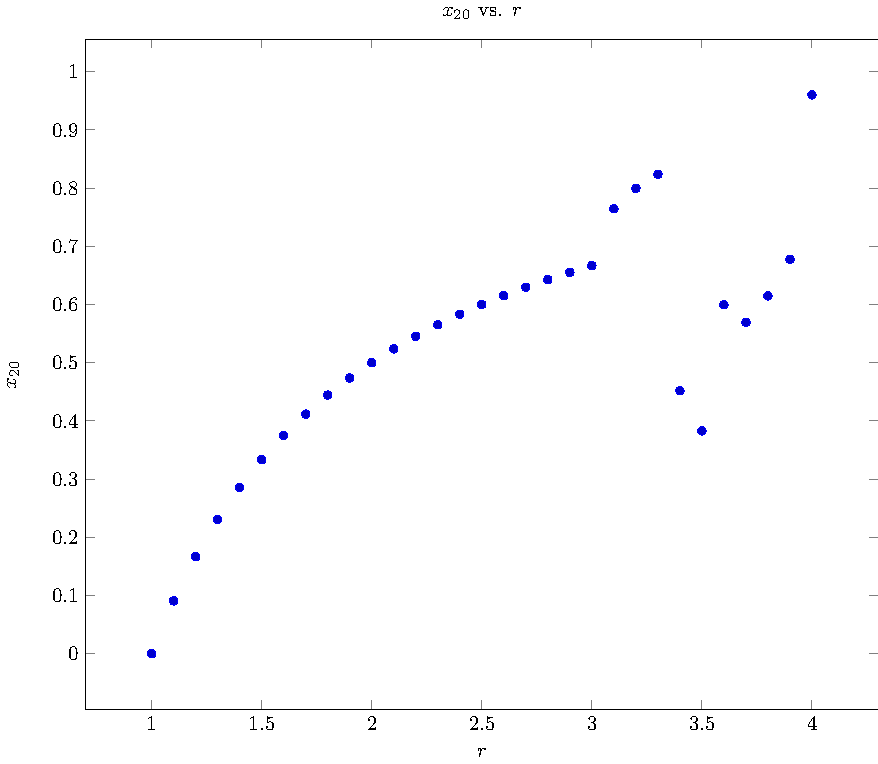
\includegraphics[width=1.0\textwidth]{Plots/PartE/xnVr.pdf}
  \end{center}
  \caption{The plot of \( x_n \) for several values of \( r \), where \( x_0 =
    0.7 \) and \( n = 20 \). The Julia program seen in Section \ref{cod:xnVr}
    was called with the command line arguments {\tt 0.7 20} to generate the
    values.}
  \label{gph:xnVr}
\end{figure}

\section{Water Drop Experiment}

\qq To collect chaotic data, the frequency with which drops formed at a sink was
recorded for a specified number of total drops. Six trials were conducted, and the
results are plotted below. Although the results were meant to be chaotic,
some of the trials show drops being produced at a fairly regular rate. The
trials in Figures \ref{fig:test3} and \ref{fig:test4} produced more regular
results than the other trials; the data points exhibit less variety than in the
other plots, which, although they are less than totally chaotic, scatter fairly
widely. 

% plots 1 and 2
\begin{figure}[H]
\centering
\begin{minipage}{.5\textwidth}
  \centering
  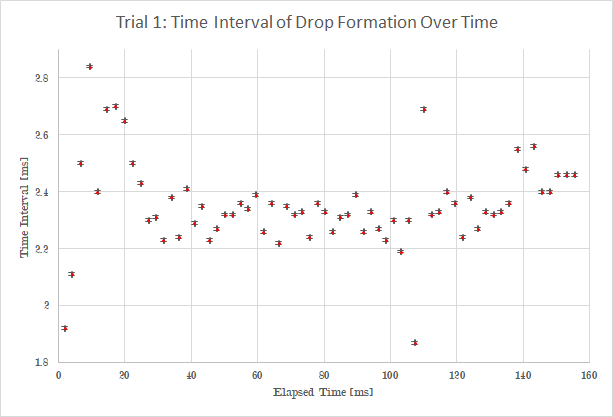
\includegraphics[width=\linewidth]{sink1.png}
  \captionof{figure}{Trial 1}
  \label{fig:test1}
\end{minipage}%
\begin{minipage}{.5\textwidth}
  \centering
  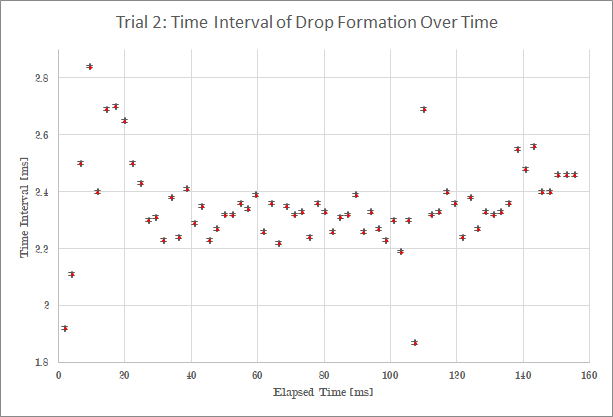
\includegraphics[width=\linewidth]{sink2.png}
  \captionof{figure}{Trial 2}
  \label{fig:test2}
\end{minipage}
\end{figure}

% plots 3 and 4
\begin{figure}[H]
\centering
\begin{minipage}{.5\textwidth}
  \centering
  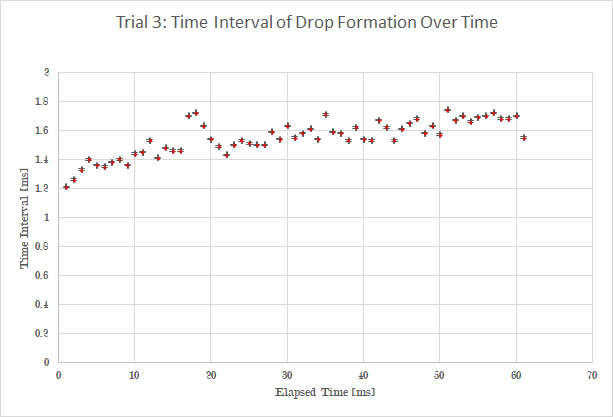
\includegraphics[width=\linewidth]{sink3.png}
  \captionof{figure}{Trial 3}
  \label{fig:test3}
\end{minipage}%
\begin{minipage}{.5\textwidth}
  \centering
  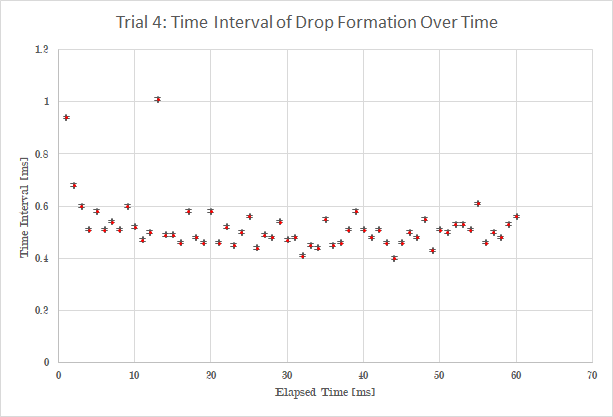
\includegraphics[width=\linewidth]{sink4.png}
  \captionof{figure}{Trial 4}
  \label{fig:test4}
\end{minipage}
\end{figure}

% plots 5 and 6
\begin{figure}[H]
\centering
\begin{minipage}{.5\textwidth}
  \centering
  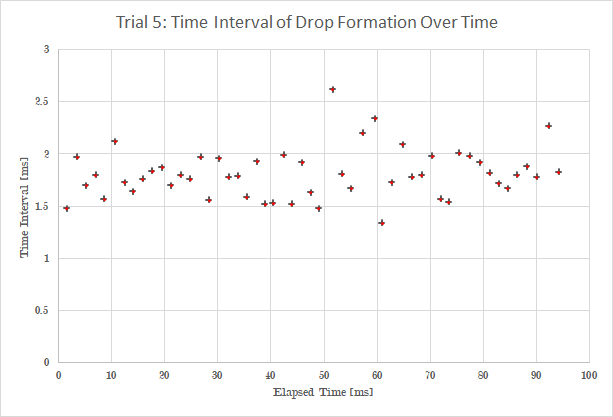
\includegraphics[width=\linewidth]{sink5.png}
  \captionof{figure}{Trial 5}
  \label{fig:test5}
\end{minipage}%
\begin{minipage}{.5\textwidth}
  \centering
  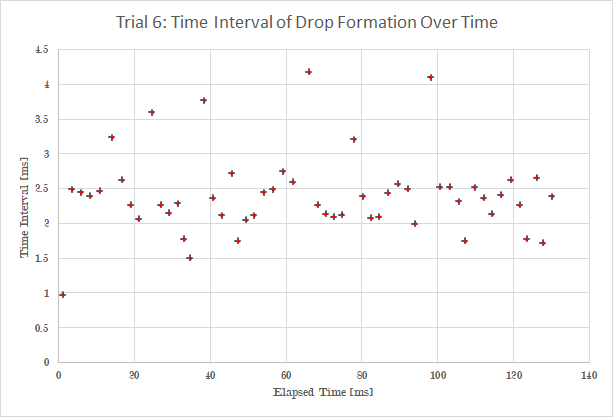
\includegraphics[width=\linewidth]{sink6.png}
  \captionof{figure}{Trial 6}
  \label{fig:test6}
\end{minipage}
\end{figure}

\section{Sources of Error}

\qq The only source of error in the experiment is present in the times at which
the water drops formed at the sink. This is random error in measurement because
it is dependent upon the reaction time of the observer. It has the nominal
effect of introducing slightly more chaos than there otherwise would have been. 

\section{Conclusion}
%Brief summary, discussion of results and theory
\qq 

\section{Appendices}

\subsection{Appendix A: Source Code}

\subsubsection{Lyapunov Exponent Calculation}
\label{cod:lyapunov}
%Lyapunov.jl

\subsubsection{\( x_n \) Calculations for Different \( r \)s}
\label{cod:xnVr}
%xnVr.jl

\end{document}
